% chapters/seismo.tex
%
% Copyright 2022 Alexander Lyttle.
%
% This work may be distributed and/or modified under the conditions of the
% LaTeX Project Public License (LPPL) version 1.3 or later.
%
% The latest version of this license is in
% https://www.latex-project.org/lppl.txt and version 1.3 or later is part of
% all distributions of LaTeX version 2005/12/01 or later.
%
%
\chapter[Asteroseismology]{Asteroseismology of Solar-Like Oscillators}

Several decades ago, 5-minute oscillations of solar surface radial velocity were observed by \citet{Leighton.Noyes.ea1962}, leading to the inference of acoustic waves trapped beneath the solar photosphere \citep{Ulrich1970}. A further decade of study culminated in the measurement of individual oscillation modes in the Doppler radial velocity \citep{Claverie.Isaak.ea1979} and total irradiance \citep{Woodard.Hudson1983a} of the Sun. Initially thought to be short-lived irregularities on the surface, these modes were found to be compatible with stochastically excited standing waves penetrating deep into the Sun. Later, \citet{Deubner.Gough1984} introduced the word \emph{helioseismology}, analogous to (geo)seismology, to describe the study of the solar interior using observations of these modes. Helioseismology was soon responsible for breakthrough solar research, from measuring differential rotation \citep{Deubner.Ulrich.ea1979} to solving the mismatch between predicted and measured solar neutrino production \citep{Bahcall.Ulrich1988}.

Astronomers initially debated the mechanism driving solar oscillation modes attributed to standing pressure waves (so-called \emph{p-modes}). \citet{Goldreich.Keeley1977} suggested what became the prevailing theory, that the p-modes were stochastically excited by near-surface convection. Hence, we might expect solar-like oscillations to be present in other stars which have a convective envelope similar to the Sun. Shortly after, \citet{Christensen-Dalsgaard1984} introduced the term \emph{asteroseismology} --- the study of the internal structure of stars with many oscillation modes present.  Shortly thereafter, solar-like oscillations were discovered in a few bright stars. Among the first solar-like oscillators discovered were Procyon and \(\alpha\) Cen A \citep{Gelly.Grec.ea1986}, with individual modes later resolved by \citet{Martic.Schmitt.ea1999} and \citet{Bouchy.Carrier2001} respectively.

% in \(\varepsilon\) Eri \citep{Noyes.Baliunas.ea1984}

% \citet{Christensen-Dalsgaard1982} suggested that the limited precision of the radial velocity method made observing solar-like oscillations in many other stars difficult.
Instrumental and atmospheric noise limited the progress of asteroseismology with ground-based equipment to studies of small number of bright dwarf stars. Asteroseismology requires high-cadence (\(\sim \SIrange{1}{10}{\minute}\)) brightness observations over long time-periods (\(\sim \SI{1}{\year}\)) with precisions of \todo{precision}. The first space-based missions which met these requirements arrived in the late 2000s, accelerating progress in the field. Initially, \emph{CoRoT} \citep{Baglin.Auvergne.ea2006} detected solar-like oscillations in thousands of red giant stars \citep{DeRidder.Barban.ea2009,Mosser.Belkacem.ea2010}. Next, \emph{Kepler} \citep{Borucki.Koch.ea2010} found oscillations in thousands more red giants \citep{Pinsonneault.Elsworth.ea2014,Pinsonneault.Elsworth.ea2018} and hundreds of main sequence stars similar to the Sun \citep{Serenelli.Johnson.ea2017}. Most recently, \emph{TESS} \citep{Ricker.Winn.ea2015} has added thousands more dwarf and giant stars to the roster of solar-like oscillators \citep[e.g.][]{Hatt.Nielsen.ea2023}. The extra constraint from asteroseismology has lead to improved stellar ages and masses... 

\begin{figure}[tb]
    \centering
    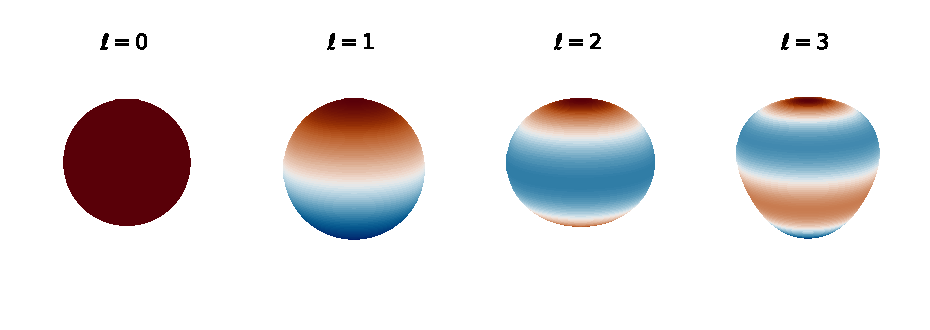
\includegraphics[trim={0 0.4in 0 0},clip]{figures/spherical_harmonics.pdf}
    \caption{Spherical harmonic oscillation modes for a few angular degrees ($l$) with azimuthal order \(m=0\). The colour-map represents the radial displacement at the surface, with \emph{blue} and \emph{red} corresponding to displacement outward and inward respectively. These regions oscillate between blue and red, with the white regions representing stationary nodes.}
    \label{fig:spherical-harmonics}
\end{figure}

The so-called p-modes are solutions to standing acoustic waves trapped inside a star, governed by its interior physics and structure. These spherical harmonic oscillators have unique frequency solutions for integers (\(n, l\)). The radial order (\(n\)) is proportional to the number of radial nodes and the angular degree (\(l\)) is the number of nodes on a given spherical shell of the star. We show a representation of the surface spherical harmonics for the first four angular degrees in Figure \ref{fig:spherical-harmonics}. For each \(l\), there exists \(2l+1\) solutions with different azimuthal order (\(m\)) corresponding to the different orientations of the nodes over the spherical shell.

\begin{figure}[tb]
    \centering
    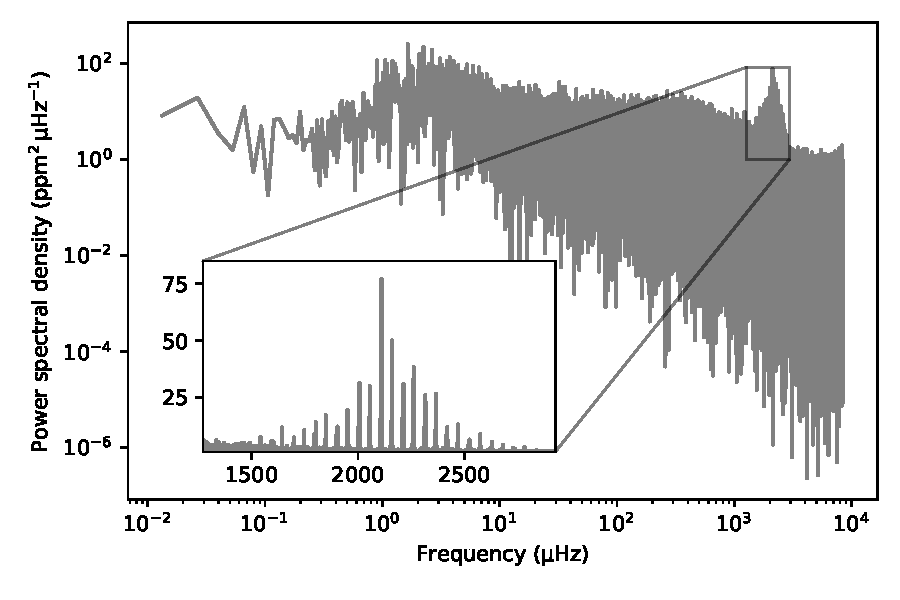
\includegraphics{figures/seismo-psd.pdf}
    \caption{The power spectral density of 16 Cyg A. The inset plot highlights the Gaussian-like power excess in the larger plot.}
    \label{fig:seismo-psd}
\end{figure}

In solar-like oscillators, p-modes are driven by near-surface convection. Typically, the timescale of this process drives high-order modes (\(n \sim 20\)). We can identify these modes in a frequency-power spectrum derived from photometric or radial velocity time series observations. For instance, both stars in the 16 Cyg system are solar-like oscillators with similar properties to the Sun \needcite. Using 16 Cyg A as an example, we downloaded the power spectrum determined by the \emph{Kepler} Asteroseismic Science Operations Centre (KASOC) using \emph{Kepler} observations\footnote{\url{https://kasoc.phys.au.dk}}. Shown in Figure \ref{fig:seismo-psd}, the power spectrum of 16 Cyg A has a distinct power excess around \SI{2000}{\micro\hertz}. We call the centre of this excess the frequency at maximum power, \(\numax\). Proportional to near-surface conditions, \citet{Brown.Gilliland.ea1991} suggested \(\numax\) scales with the acoustic cut-off frequency --- the highest frequency at which acoustic waves can reflect near the stellar surface.

Looking closely at the power excess in Figure \ref{fig:seismo-psd}, we can see a comb of evenly spaced peaks. But what do these represent, what information to they hold?

Different angular degrees probe different depths into the star. With the Sun, the surface can be resolved allowing for high angular degree modes to be studied. However, integrating over the solar surface, high angular degree modes cancel out leaving only \(l \lesssim 3\) detectable \needcite.

In the case of a rotating or asymmetric star, the observed mode frequencies split for different \(m\) via the Doppler effect. However, we hereafter consider the case of a slowly rotating, spherically symmetric star, such that solutions of different \(m\) are approximately the same frequency.

If we consider an acoustic wave in a one-dimensional homogeneous medium, then we would expect each mode of oscillation to be an integer multiple of the fundamental mode. While the case for a star is more complicated, we can also approximate the frequencies for different modes as a multiple of some characteristic frequency. \citet{Tassoul1980} found that the mode frequencies could be approximated by assuming the asymptotic limit where \(l/n \rightarrow 0\), giving the following following expression \citep{Gough1986},
%
\begin{equation}
    \nu_{nl} \simeq \left(n + \frac{l}{2} + \varepsilon\right) \nu_0 + \mathcal{O}(\nu_{nl}^{-1}), \label{eq:asy}
\end{equation}
%
where \(\varepsilon\) is some constant offset. The characteristic frequency \(\nu_0\) is the inverse of the acoustic diameter,
%
\begin{equation}
    \nu_0 = \left(2 \int_{0}^{R} \frac{\dd r}{c(r)}\right)^{-1},
\end{equation}
%
where \(c(r)\) is the sound speed as a function of radius (\(r\)) and \(R\) is the stellar radius. \citet{Gough1986} found that similarly to other variable stars, this characteristic frequency relates to the mean density by \(\nu_0 \propto \overline{\rho}^{\,1/2}\). While \(\nu_0\) is not directly detectable in solar-like oscillators, we can approximate it by taking the difference between consecutive modes of the same angular degree, \(\Delta\nu_{nl} = \nu_{nl} - \nu_{n-1\,l}\). Therefore, estimates of a global (or average) \(\Delta\nu\) provides information about the density of a star, leading to improved constraint on its mass and radius.

\begin{figure}[tb]
    \centering
    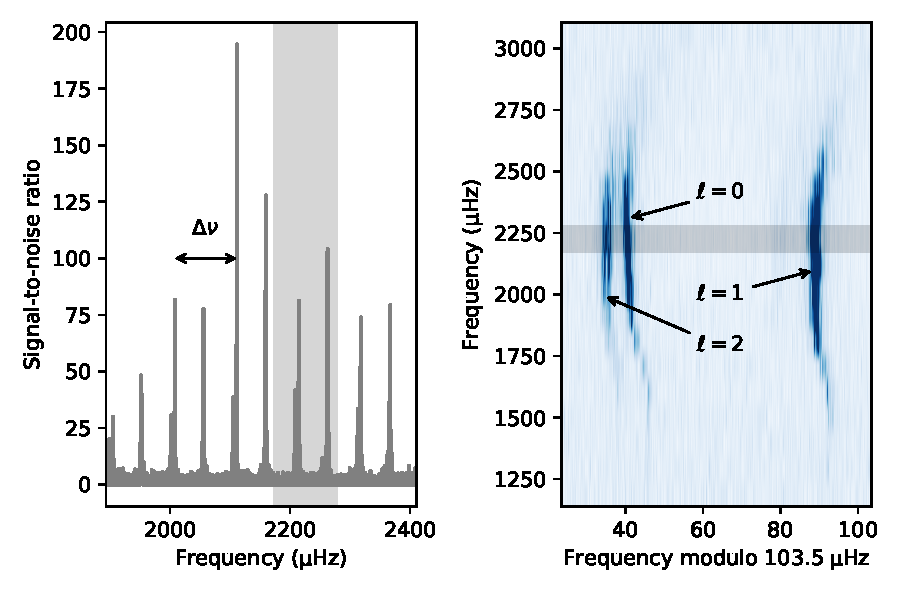
\includegraphics{figures/seismo-echelle.pdf}
    \caption{\emph{Left:} A section of the spectral signal-to-noise ratio (SNR) against frequency for 16 Cyg A. The large frequency spacing (\(\Delta\nu\)) between two radial modes is annotated with a double-headed arrow. The shaded region corresponds to a single row (also highlighted) in the echelle plot (\emph{right}). The echelle plot shows the spectral SNR such that a darker colour represents a higher SNR. Each row spans \SI{103.5}{\micro\hertz} and is stacked in order of frequency. The apparent ridges are labelled according to the angular degree (\(l\)) of the modes they represent.}
    \label{fig:seismo-echelle}
\end{figure}

The asymptotic expression helps us identify modes in a star. If Equation \ref{fig:asy} was exact, we would expect odd and even modes to oscillate at the same frequencies. To see this, we return to the power spectrum of 16 Cyg A with an estimate of the noise divided out. We can see the regular pattern predicted by Equation \ref{fig:asy} in the left panel of Figure \ref{fig:seismo-echelle}. Every other mode is approximately separated by \(\dnu\). To see this effect over the wider spectrum, we created an \emph{echelle} plot in the right panel. Folding the spectrum by an estimate of \(\dnu\), reveals a sequence of ridges corresponding to modes of different angular degree. Odd and even angular degree are grouped together, although do not lie on top of each other.

% The 16 Cyg binary star system is home to two well-studied solar-like oscillators. As an example of what these observations look like, we will consider 16 Cyg A. Observed by \emph{Kepler} \todo{details like quarters}, the Kepler Asteroseismic Science Operations Center (KASOC\footnote{\url{https://kasoc.phys.au.dk}}) processed the light curve to extract the oscillation power spectrum. The details of their data reduction and processing can be found in \needcite. Briefly, creating a periodogram using the Lomb-Scargle method \citep{Lomb1976,Scargle1982}. We show the full power spectrum in Figure \ref{fig:seismo-psd}. We can see a clear Gaussian-like bump at around \SI{2000}{\micro\hertz}. Enlarging this, we see that it comprises a repeating patten of equally-spaced peaks.

% The comb of peaks in the power spectrum corresponds to oscillation modes in the star. In Figure \ref{fig:seismo-echelle}, we show a small section of the power section with an estimate of the noise divided out. We see a regular repeating pattern, with similar modes repeated by approximately \(\Delta\nu\). If we wrap the spectrum by \(\Delta\nu\), we get the so-called echelle diagram. Ridges of high SNR correspond to modes of different angular degree. From the asymptotic expression, we expect modes of even angular degree grouped together, and likewise for odd angular degrees.

How can asteroseismology tell us about the star? Globally, we can use the scaling relations.

We can also use individual modes and compare with models. Worth noting the surface term here.
